\documentclass[12pt]{article}
\usepackage{graphicx}
\usepackage{float}
\usepackage{amsmath}
\title{Experiment 9: Clock Divider, Serial Adder}
\author{Annirudh K P\\%
210070009}
\date{October 13, 2022}
\begin{document}

\maketitle

\section{Overview of the experiment}
\paragraph{}
In this experiment, we worked on some sequential circuit designs using behavourial modelling on VHDL. The problem statement of this experiment is to design a Clock Divider as well as a bonus question of Serial Adder. The objective of this experiment was to understand the Quartus Design Flow, work with the Xen10 Board, use Pin Planning, and give us hands on experience over different technical glitches/problems we may face in this piece of software which has been made unwantedly hard.

\section{Experimental Set-up}

\subsection{Design Schematics}
The idea behind the design of Clock divider is shown:

\begin{figure}[H]
\centering
  \includegraphics*[scale=0.7]{Images/ClockDiv_Design.jpeg}\
\end{figure}

The following state diagram is shown for the Serial Adder

\begin{figure}[H]
\centering
  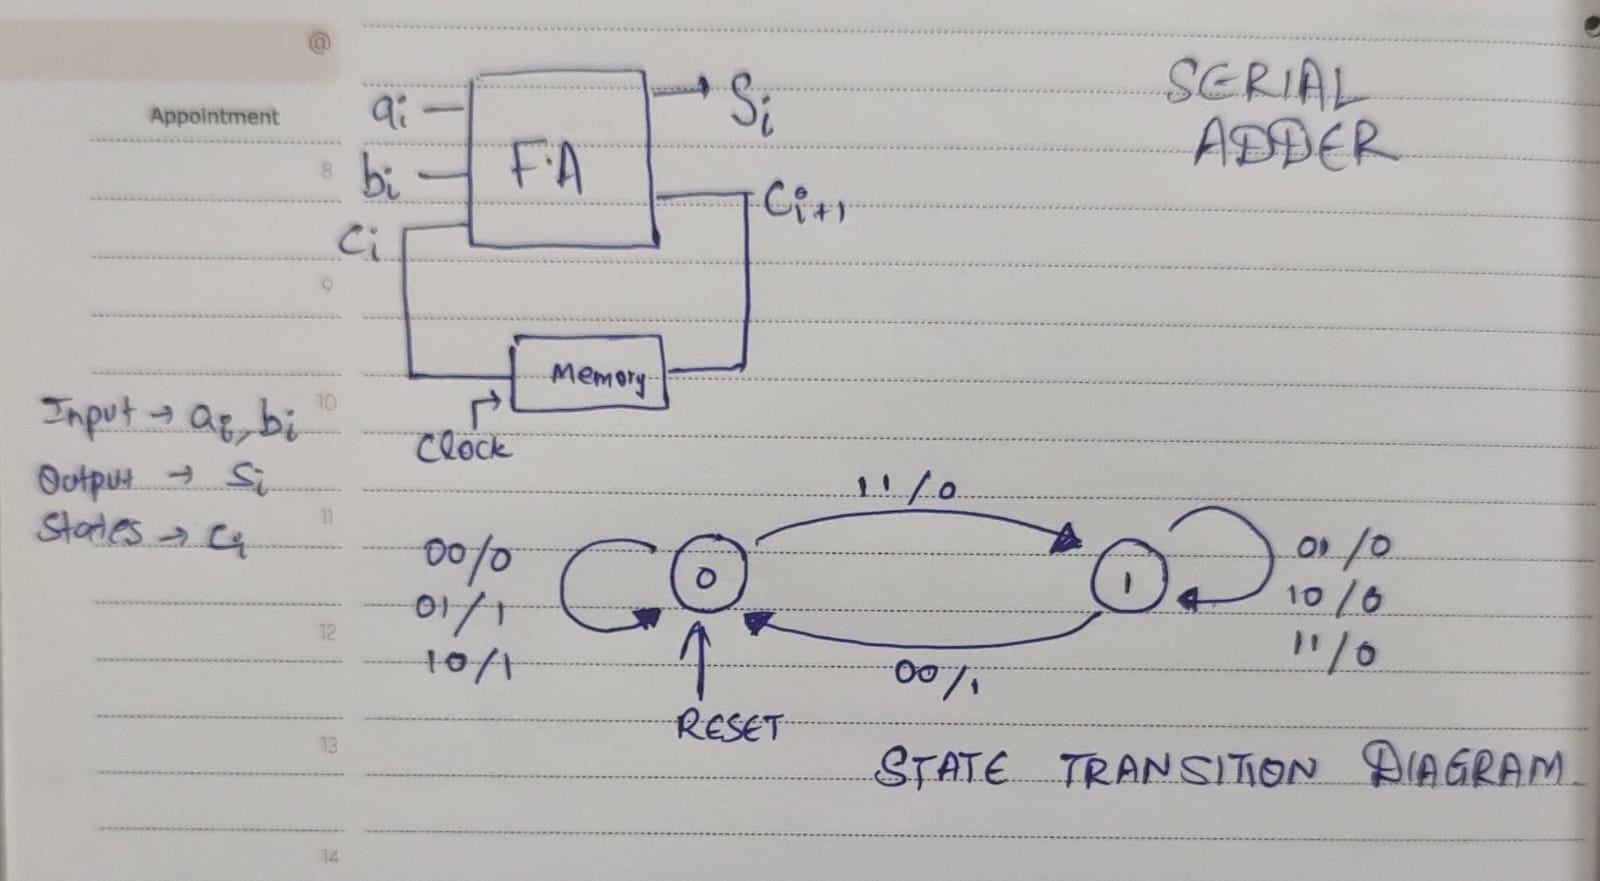
\includegraphics[scale=0.3]{Images/SerialAdder_Design.jpeg}
  \caption{}
\end{figure}

\subsection{Description of Components}
\subsubsection{Clock Divider}
\begin{verbatim}
library ieee;
use ieee.std_logic_1164.all;
use ieee.numeric_std.all;

entity clock_divider is
port (clk_out : out std_logic;
		clk_50, resetn : in std_logic);
end entity clock_divider;

architecture bhv of clock_divider is
signal count : integer := 1;
signal clk_out_temp : std_logic := '1';

begin
clock_proc:process(clk_50,resetn)
begin
	if(clk_50='1' and clk_50' event) then
		count <= count + 1;
	end if;
	
	if (count = 50000000) then
		count <= 1;
		--clk_out <= not clk_out_temp;
		clk_out_temp <= not clk_out_temp;
	end if;
		
	if (resetn = '0') then 
		count <= 1;
		--clk_out <= '1';
	end if;
	clk_out <=  clk_out_temp;
end process;
end bhv;
\end{verbatim}

\subsubsection{Serial Adder}
\begin{verbatim}
library ieee;
use ieee.std_logic_1164.all;
use ieee.numeric_std.all;

entity Serial_Adder is
	port (reset, a, b, clock: in std_logic; s: out std_logic);
end entity;

architecture bhv of Serial_Adder is

type state is (s0, s1); 
signal y_present,y_next: state:=s0;
signal sd1: std_logic;

begin
clock_proc:process(clock,reset)
begin
	if(clock='1' and clock' event) then
		if(reset = '1') then
			y_present<=s0;
			sd1 <= '0';
		else
			sd1 <= '1';
			y_present<=y_next;
		end if;
	end if;
end process;

state_transition_proc:process(a,b,y_present)
begin
	if (clock='1' and clock' event) then
		case y_present is
			when s0=>
				if(a='1' and b ='1') then
					y_next <= s1;
				else
					y_next <= s0;
				end if;
			when s1=>
				if(a='0' and b ='0') then 
					y_next <= s0;
				else
					y_next <= s1;
				end if;
			when others=>
				null;
		end case;
	end if;
end process;

output_proc:process(y_present, a, b) 
begin
	case y_present is
		when s0=>
			if ((a='0' and b ='1') or (a='1' and b='0')) then
				s<=('1' and sd1);
			else 
				s<=('0' and sd1);
			end if;
		when s1=>
			if ((a='0' and b ='0') or (a='1' and b='1')) then
				s<=('1' and sd1);
			else 
				s<=('0' and sd1);
			end if;
		when others=>
			null;
	end case;
end process;

end bhv;
\end{verbatim}

\section{Observations}
 
We get RTL simulation waveforms for corresponding to input and output which is given below and it shows required results.

\begin{figure}[H]
\centering
  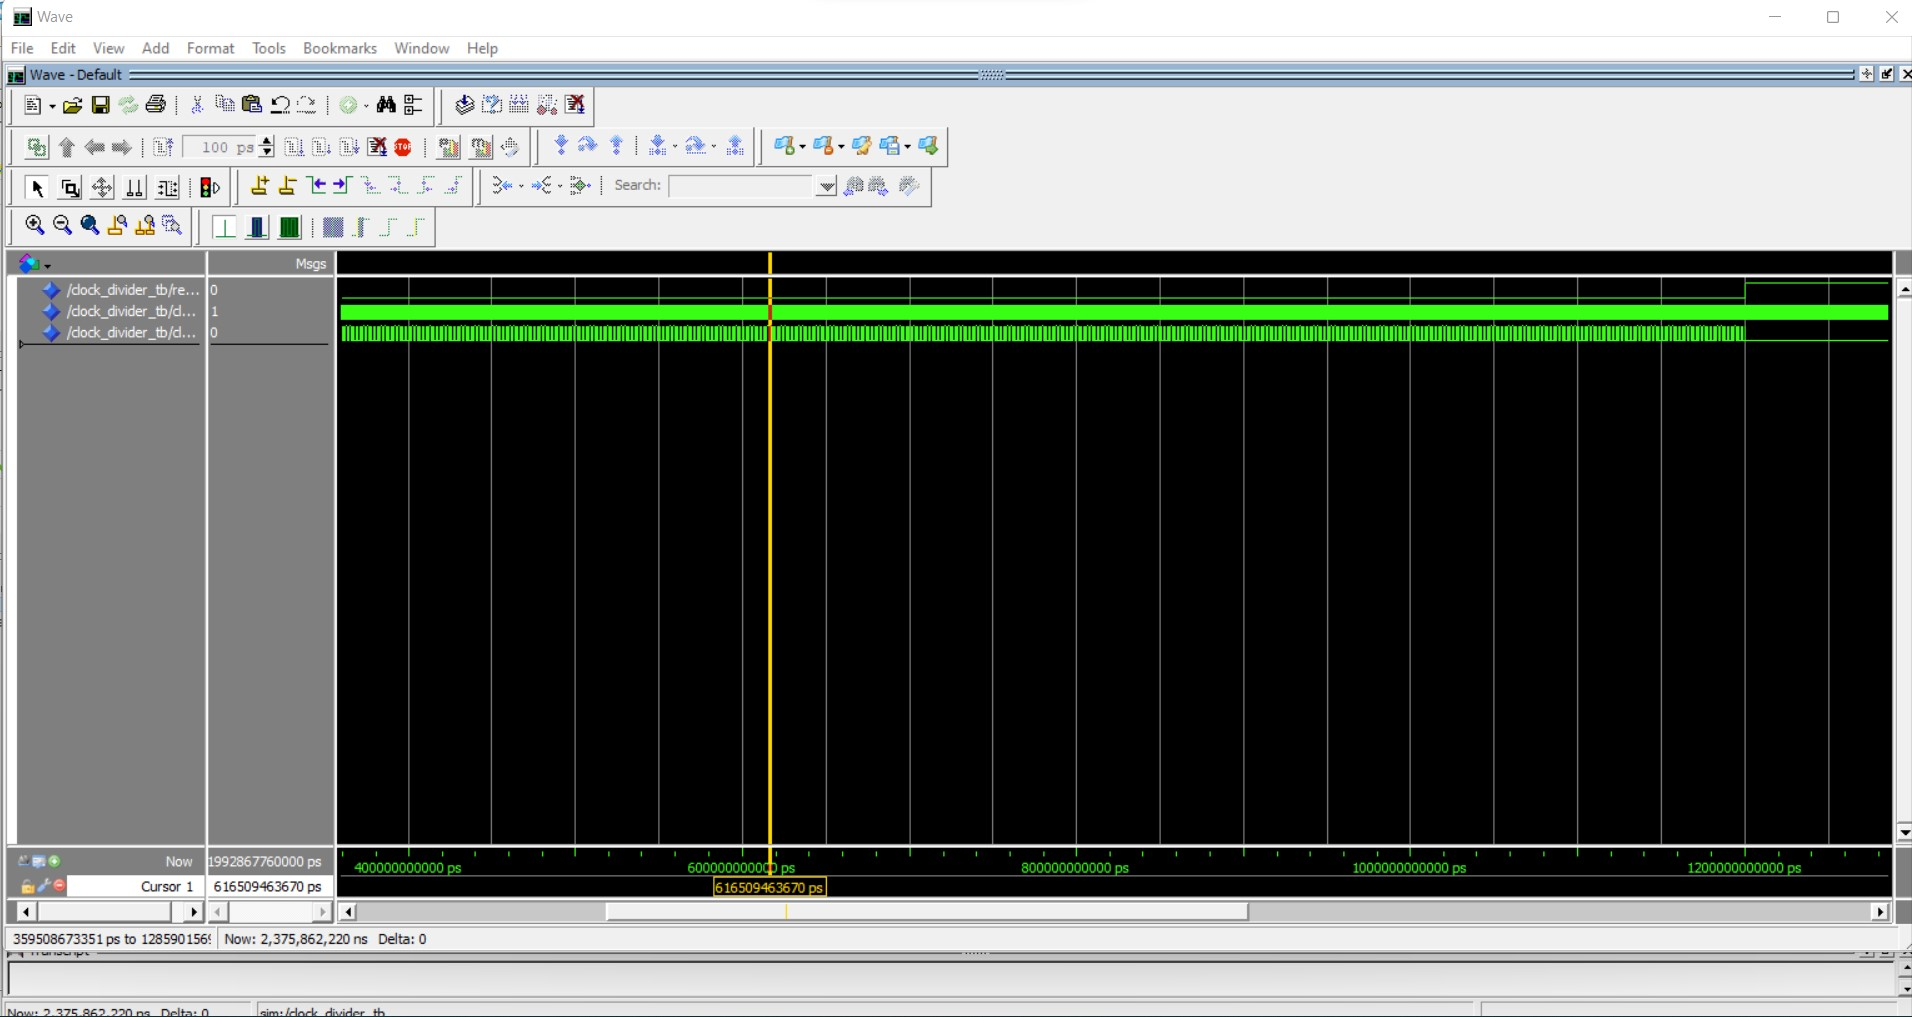
\includegraphics[scale=0.35]{Images/ClockDiv480Hz_RTLSimulation.jpeg}
  \caption{Clock Divider RTL Simulation - 480 Hz}
\end{figure}

\begin{figure}[H]
\centering
  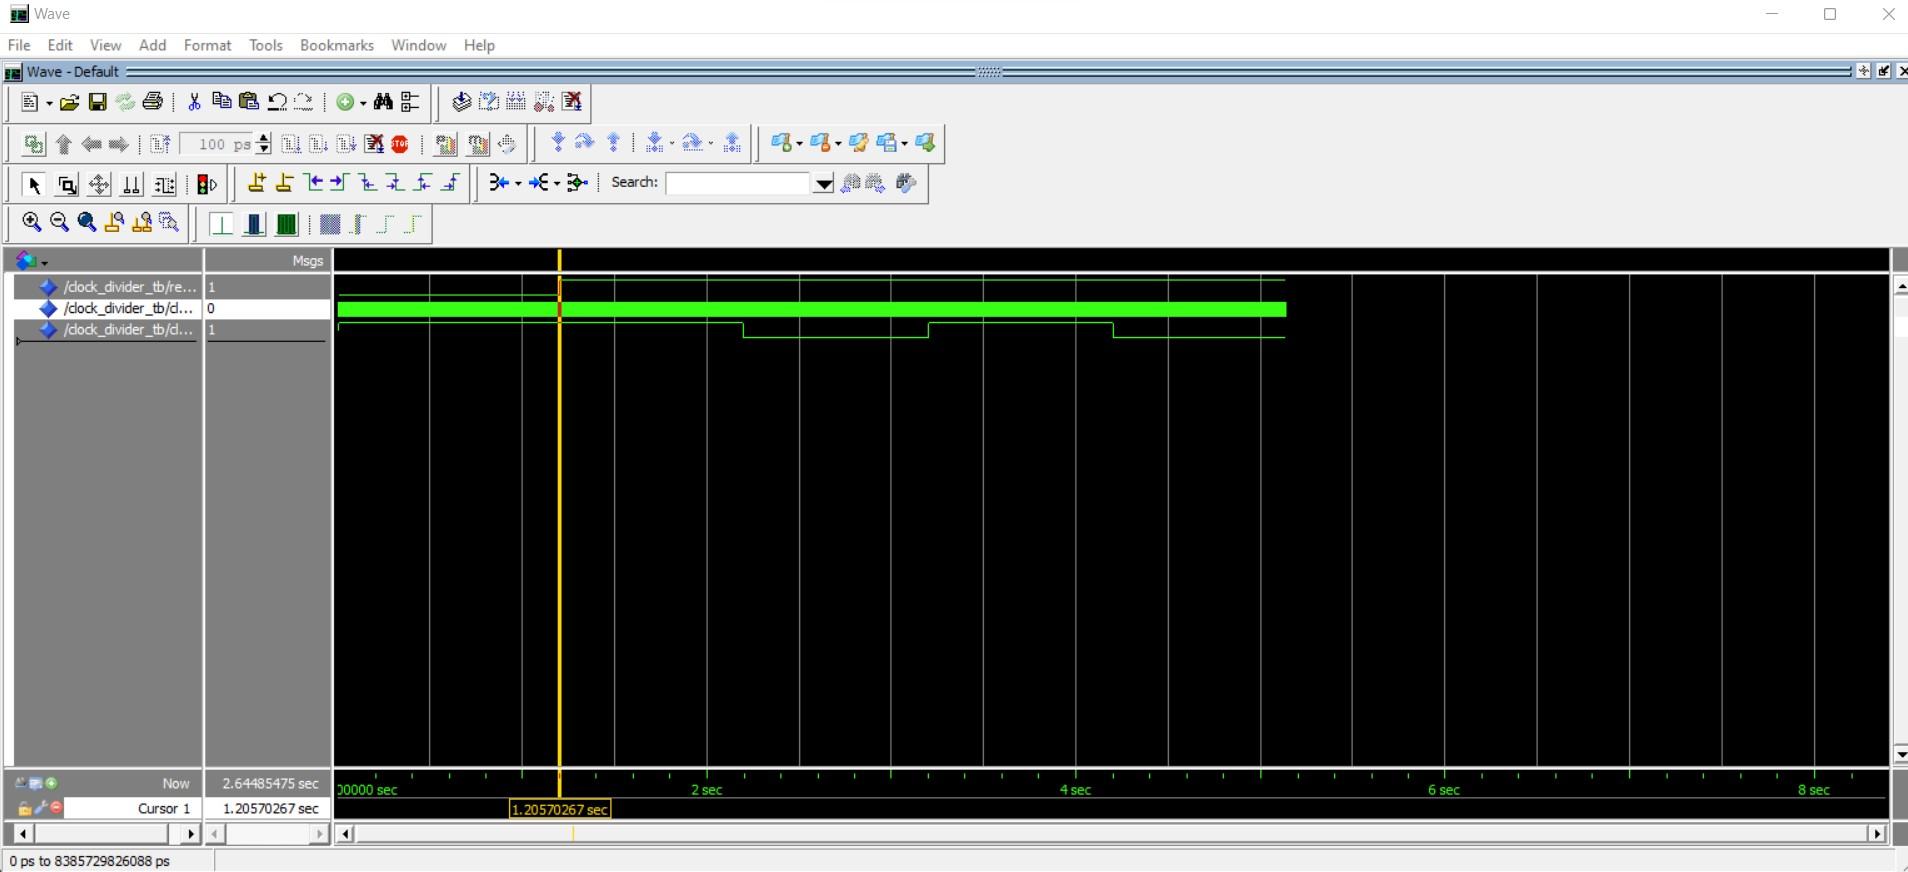
\includegraphics[scale=0.35]{Images/ClockDiv0.5Hz_RTLSimulation.jpeg}
  \caption{Clock Divider RTL Simulation - 0.5 Hz}
\end{figure}

Further the code after appropriate pin planning, (in form of .svf file) was flashed onto the Xen10 board. Then was run to generate a blinking LED output. The output was verified, which also verified the working of the logic for the Clock Divider.

Also the bonus question of Serial Adder was successfully implemented and RTL Simulation was run, with all test cases being passed.

\begin{figure}[H]
\centering
  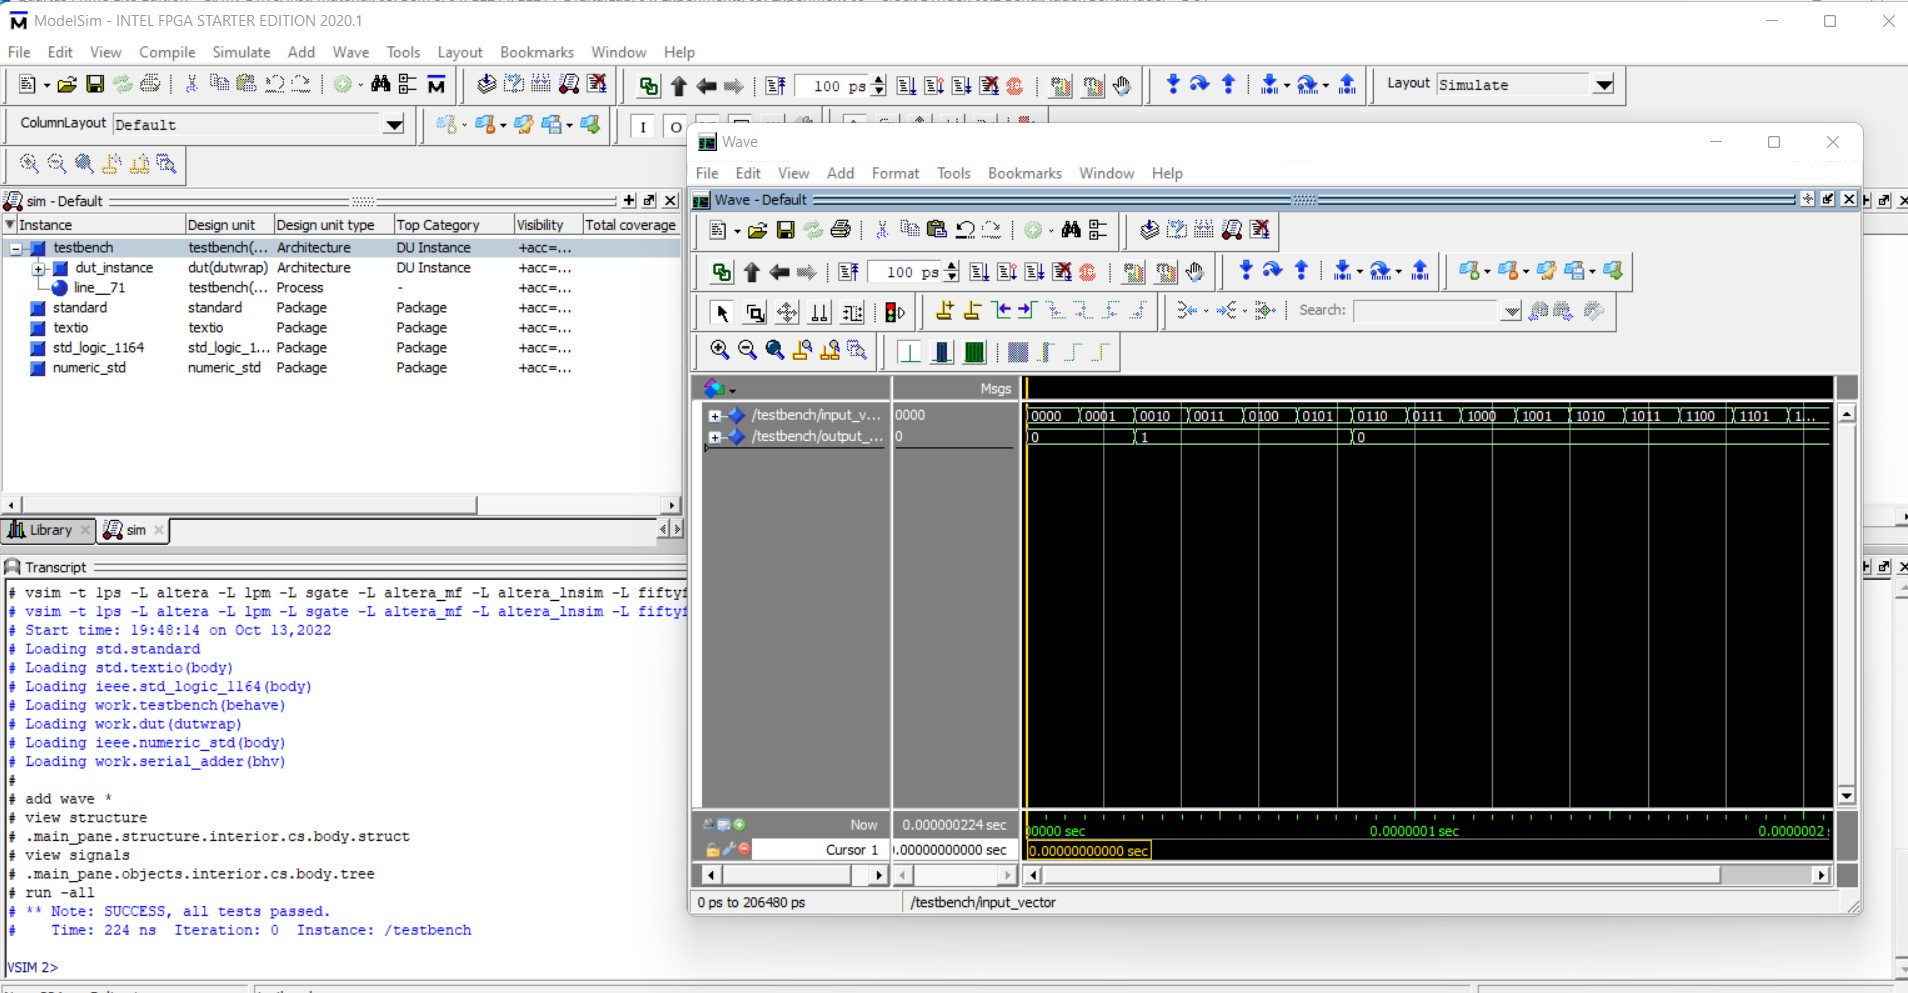
\includegraphics[scale=0.35]{Images/SerialAdder_RTLSimulation.jpeg}
  \caption{Serial Adder RTL Simulation}
\end{figure}

\end{document}